%-------------------------------------------------------------------------------------------------------------------------------------
%                                                   BIOGRAPHY
%-------------------------------------------------------------------------------------------------------------------------------------
\vspace{2.0cm}
\begin{IEEEbiography}[{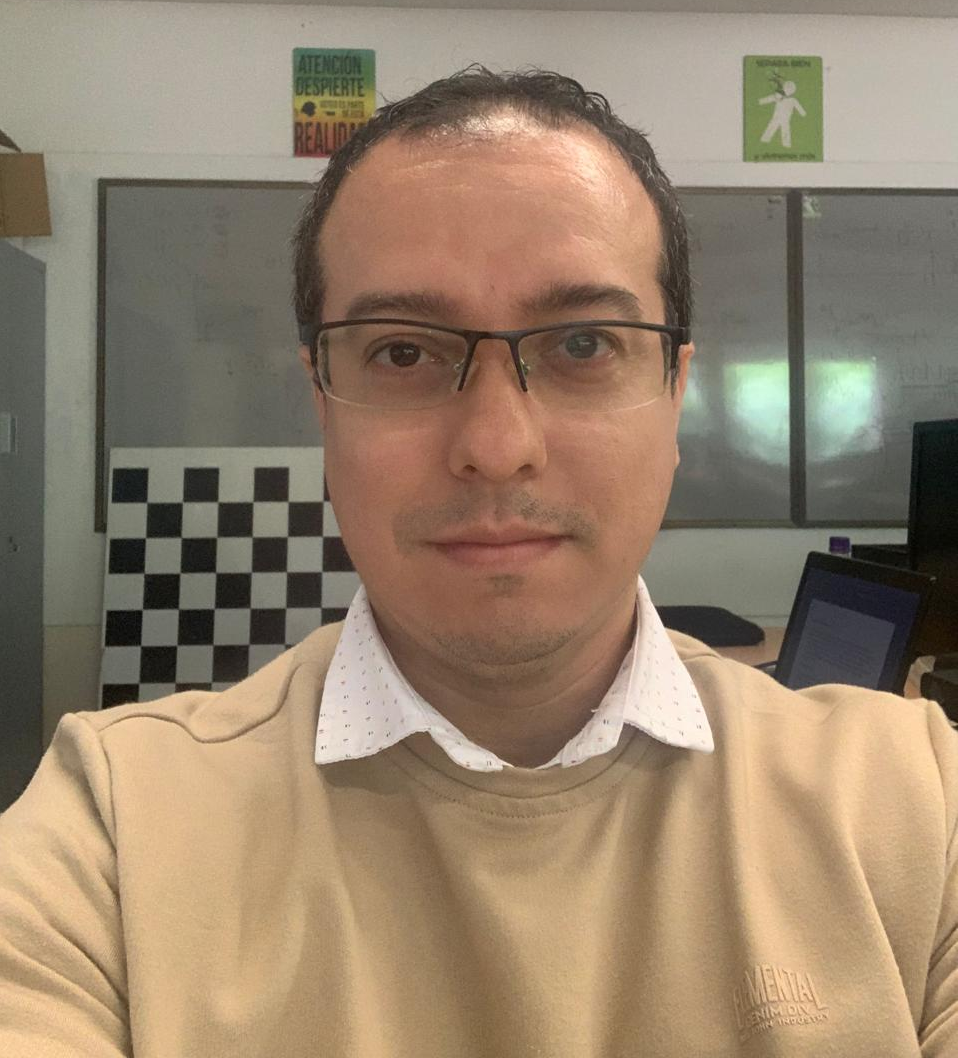
\includegraphics[width=1in,height=1.25in,clip,keepaspectratio]{Figures/Photo_AANP.png}}]{Alvaro Navarro-Perez}
    (Member, IEEE) received the B.Sc. degree in Electronic Engineering from the Universidad del Quindío, Colombia, in 2008, and the M.Sc. degree in Robotics and Automation from TU Dortmund University, Germany, in 2015. He is currently pursuing the Ph.D. degree in Engineering at the Universidad del Valle, Colombia.
    He is an Assistant Professor with the Faculty of Engineering, Universidad del Quindío. He is also a member of the IEEE Robotics and Automation Society (RAS) and the Technological Development Research Group (GIDET). His research interests include instrumentation systems, autonomous robots and localization and mapping for self-driving cars. His current research focuses on semantic mapping for long-term localization using multi-modal systems.
\end{IEEEbiography}
\vspace{-2.0cm}
\begin{IEEEbiography}[{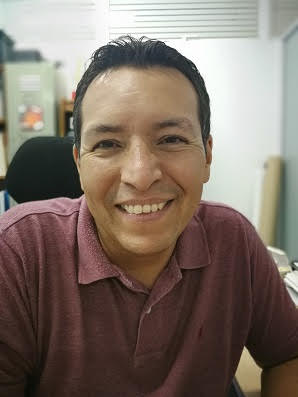
\includegraphics[width=1in,height=1.25in,clip,keepaspectratio]{Figures/Photo_BBC.jpg}}]{Bladimir Bacca-Cortes}
    received the degree in electronic engineering and the master’s degree in automation from the Universidad del Valle, Valle del Cauca, Cali, Colombia, in 1999 and 2004, respectively, and the Ph.D. degree in technology from the Universitat de Girona, Cataluña, Girona, Spain, in 2012. He is currently a Full Professor with the School of Electrical and Electronic Engineering, Universidad del  Valle. He is a member of the research group on Perception and Intelligent Systems. His research interests include mobile robotics, simultaneous localization and mapping systems, and computer vision
\end{IEEEbiography}
\vspace{-2.0cm}
\begin{IEEEbiography}[{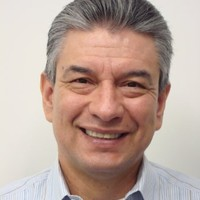
\includegraphics[width=1in,height=1.25in,clip,keepaspectratio]{Figures/Photo_ECB.jpg}}]{Eduardo Caicedo-Bravo}
    received the degree in electronic engineering and the master’s degree in automation from the Universidad del Valle, Valle del Cauca, Cali, Colombia, in 1985 and 1993, respectively, and the Ph.D. degree in Engineering from the Polytechnic University of Madrid-Spain in 1996. He is currently a Full Professor with the School of Electrical and Electronic Engineering, Universidad del  Valle. He is the director of the research group on Perception and Intelligent Systems (PSI). Author of several books and scientific articles, guest speaker at national and international events and visiting professor at international universities. He has worked projects with COLCIENCIAS, The European Union, CYTED, the Swiss Confederation and national companies. Areas of Interest: Smart Grids, Instrumentation Electronics, Intelligent Systems, Computational Intelligence and Robotics.
\end{IEEEbiography}